\section{Methods}

\subsection{Plasmid Design}

We have used the pBbB6c-GFP plasmid for all our designs. This plasmid comes with GFP mut3b CDS inducible with addition of IPTG. The original RBS for the GFP CDS was replaced with combination of PCR and isothermal assembly. Primers and the assembly strategy have been generated using the Teselagen BUILD software (Teselagen Biotechnology).

\subsection{PCR}
PCR amplification of the cloning inserts was done using Q5 High-Fidelity 2X Master Mix (NEB, catalogue no. M0492L). 20 \(\mu\)L reactions were prepared by dispensing each of the 10 \(\mu\)M reverse primers into a well of a 96-well PCR plate using the Labcyte Echo Liquid Handler. A mastermix consisting of polymerase premix, plasmid DNA template, and the single 10 forward primer was prepared by and dispensed by hand. Reactions were run using Touchdown PCR or standard PCR cycling methods in BioRad C1000 thermal cyclers. Then, samples were incubated at 37°C for 60 minutes, followed by a 20-minute heat inactivation step at 80°C.
Capillary electrophoresis of PCR products was performed using the Agilent Technologies ZAG DNA Analyzer system. 2µL of each PCR reaction was electrophoresed using the ZAG 130 dsDNA Kit (75-20000bp) or ZAG 110 dsDNA Kit (35-5000bp) (Agilent Technologies, catalogue no. ZAG-110-5000; ZAG-130-5000). ProSize Data Analysis Software (Agilent Technologies) was used to generated gel images from the sample chromatograms and sizes were estimated by reference to the upper and lower DNA markers spiked into each sample and a DNA ladder run in well H12 of each sample plate. 

\subsection{isothermal DNA Assembly}
Constructs were assembled using NEBuilder HiFi DNA Assembly Master Mix (NEB, catalogue no. E2621L). Samples were incubated at 37°C for 60 minutes, followed by a 20-minute heat inactivation step at 80°C. Reactions consisting of the common fragment and the variable fragment were prepared using the Echo acoustic liquid handler, to a final volume of 5 or 10\(\mu\)L . Assemblies were run in the thermal cycler for 1 hour at 50°C, followed by an infinite hold step at 4°C.

\subsection{\textit{E. coli} transformation}
The DH5α cell line (Thermo Fisher Scientific, catalogue no. 18265017) was made chemically competent using the Mix & Go \textit{E. coli} Transformation Kit & Buffer Set (Zymo Research, catalogue no. T3001). 20\(\mu\)L of cells was aliquoted into each well of a cold 96-well PCR plate and stored at -80°C for later use. Plates of cells were thawed on a -20°C cold block before 3µL of the assembly product was added and mixed using the CyBio FeliX liquid handler. Cells were incubated on a cold block for 2-5 minutes before being plated in a 96 square grid on Omnitrays containing LB (BD, catalogue no. ***) with 34\(\mu\)g/mL chloramphenicol (Sigma, catalogue no. ***). Multiple dilutions of cells in LB were prepared and plated in parallel on Omnitrays. Plates were incubated overnight at 37°C.

\subsection{Automated colony picking and culturing}
A Singer Instruments PIXL colony picker was used to select individual colonies from the transformation plates. Each selected colony was used to inoculate 1mL of selective medium in a 2mL square well 96 plate. They were then cultured overnight in 37°C with shaking (~300rpm).

\subsection{Glycerol stock preparation}
100µL of sterile 80\% (v/v) glycerol and 100µL of overnight culture were combined in the wells of a 96 deep (2mL) round well plate using the CyBio Felix liquid handler. They were then sealed with a 96-well silicon sealing mat and transferred to a -80°C freezer. 

\subsection{Cuture analysis}
Overnight cultures were started by inoculating 1mL of LB medium supplemented with 34\(\mu\)g/mL chloramphenicol with ~2\(\mu\)L of the glycerol stock in a 96 deep (2mL) round well plate. Cultures were incubated at 37°C with shaking (~300rpm) for ~17 hours. The following morning, 20\(\mu\)L of overnight culture was added to 980\(\mu\)L of fresh selection medium and precultures were grown at 37°C with shaking in 2mL round well 96 plate. 
After 90 minutes, two parallel cultures were prepared in flat-bottom clear polystyrene 96-well plates and were induced with 500\(\mu\)M IPTG – one plate of 300\(\mu\)L cultures for flow cytometry analysis (induced with 1.5\(\mu\)L of 0.1M IPTG) and one plate of 200\(\mu\)L cultures for plate reader analysis (induced with 1.0\(\mu\)L of 0.1M IPTG).
•	Cytation 5 acquisition and incubation/shaking settings
•	CytoFLEX S acquisition settings

\subsection{Machine learning experimental design}

To automatically design the RBS sequences in batch using machine learning, we need to consider two parts: 
1) Design an regression algorithm which takes the RBS sequences as input and returns the predicted TIR scores and the confidence intervals for the said predictions. 
2) Design an online learning approach which recommends the RBS sequences based on the predicted TIR scores and confidence intervals. 
Such online learning approach provides the $\textit{exploitation-exploration balance}$ that we use to control our machine learning process.

Specifically, since our goal is to find a RBS sequence with the largest possible TIR score after the total number of rounds $N$,  we consider our experimental design problem as one of sequentially optimising an unknown reward function $f: \mathcal{D} \rightarrow \mathbb{R}$, where $\mathcal{D}$ is the set containing all RBS sequence points, and $f(\mathbf{x})$ is the TIR score at $\mathbf{x}$. 
In each round $t$, we choose a set of $m$ points $\mathcal{S}_t \subset \mathcal{D}$ and observe the function values of each points in the selected set $\mathcal{S}_t$, i.e. $y_i = f(\mathbf{x}_i) + \epsilon_i$, for all $i \in \mathcal{S}$, where $\epsilon_i$ is the noise (we assume the noise is following Gaussian distribution with unknown mean and variance). This noise is influenced by the accuracy of the RBS predictor and other experimental interference (e.g. \textcolor{red}{To be added}). 


\begin{itemize}
    \item \textit{Gaussian process regression (GPR)}.
    A Gaussian process regression model \cite{Rasmussen2004} is a Bayesian approach to regression which provides uncertainty measurements on predictions. 
    We model $f$ as a sample from a \textit{Gaussian process} $GP(\mu(\mathbf{x}), k(\mathbf{x}, \mathbf{x'}))$, which is specified by the mean function $\mu(\mathbf{x})=\mathbb{E}[f(\mathbf{x})]$ and the kernel (or covariance) function $k\left(\mathbf{x}, \mathbf{x}^{\prime}\right)=\mathbb{E}[(f(\mathbf{x})-\left.\mu(\mathbf{x}))\left(f\left(\mathbf{x}^{\prime}\right)-\mu\left(\mathbf{x}^{\prime}\right)\right)\right]$.\\
    We chose to use \textit{spectrum kernel} \cite{leslie2001spectrum} to specify the kernel function of $GP$.  
    The spectrum kernel is widely used for classifying protein sequences \cite{leslie2001spectrum, ben2008support}, which takes two sequences as inputs and outputs a scalar value which represents the similarities between the two sequences. More precisely, $k_\ell^{\text{spec}}(\textbf{x}, \textbf{x}^\prime) =\left\langle\Phi_{\ell}^{\mathrm{spec}}(\mathbf{x}), \Phi_{\ell}^{\mathrm{spec}}\left(\mathbf{x}^{\prime}\right)\right\rangle$, where $\mathbf{x}, \mathbf{x}^\prime$ are two RBS sequences in $\mathcal{D}$ over an alphabet $\Sigma$. Denote the number of letters in the alphabet as $|\Sigma|$. $\Phi_{\ell}^{\mathrm{spec}}(\mathbf{x})$ maps the sequence $\textbf{x}$ onto a $|\Sigma|^\ell$ dimensional feature space, where each dimension is the count of the number of one of the $|\Sigma|^\ell$ possible strings $s$ of length $\ell$.
    %Since the sequences in provided data have the pattern that the core area is different from each other, and other areas are similar. So the kernel for Gaussian Process we are using is the sum of kernels, for core areas we use spectrum kernel with string as input directly, and for other areas we use one-hot encoding and dot product kernel for simplicity.
    
    
    \item \textit{Upper confidence bound (UCB)}. Bandit algorithms \cite{lattimore2018bandit} provide various approaches to sequential design where an agent adaptively chooses one or more options among several actions based on certain policies. In our work we used the Upper Confidence Bound version of that algorithm, which is based on the \textit{optimism in the face of uncertainty}. The UCB algorithm, as the name suggests, basically selects RBS sequences with the maximum upper confidence bound, i.e. $\operatorname{argmax}_{\mathbf{x}_i \in \mathcal{D}} \left( \mu_t(\mathbf{x}_i) + \beta_t \sigma_t(\mathbf{x}_i)\right)$,
    where $\beta_t$ is a hyperparameter balancing the exploitation and exploration, 
    $\mu_t(\mathbf{x}_i), \sigma_t(\mathbf{x}_i)$ are the predicted mean and standard deviation at round $t$ for the sequence $\mathbf{x}_i$. 
\end{itemize}

Combined the two parts together, we apply \textit{Gaussian Process Upper Confidence Bound (GPUCB)} algorithm, which has been theoretically analysed by \textcite{srinivas2012information}. We show the flowchart of machine learning based experimental design in Figure \ref{fig: flowchart of machine learning based experimental design.}.


\begin{figure}[t]
    \centering
    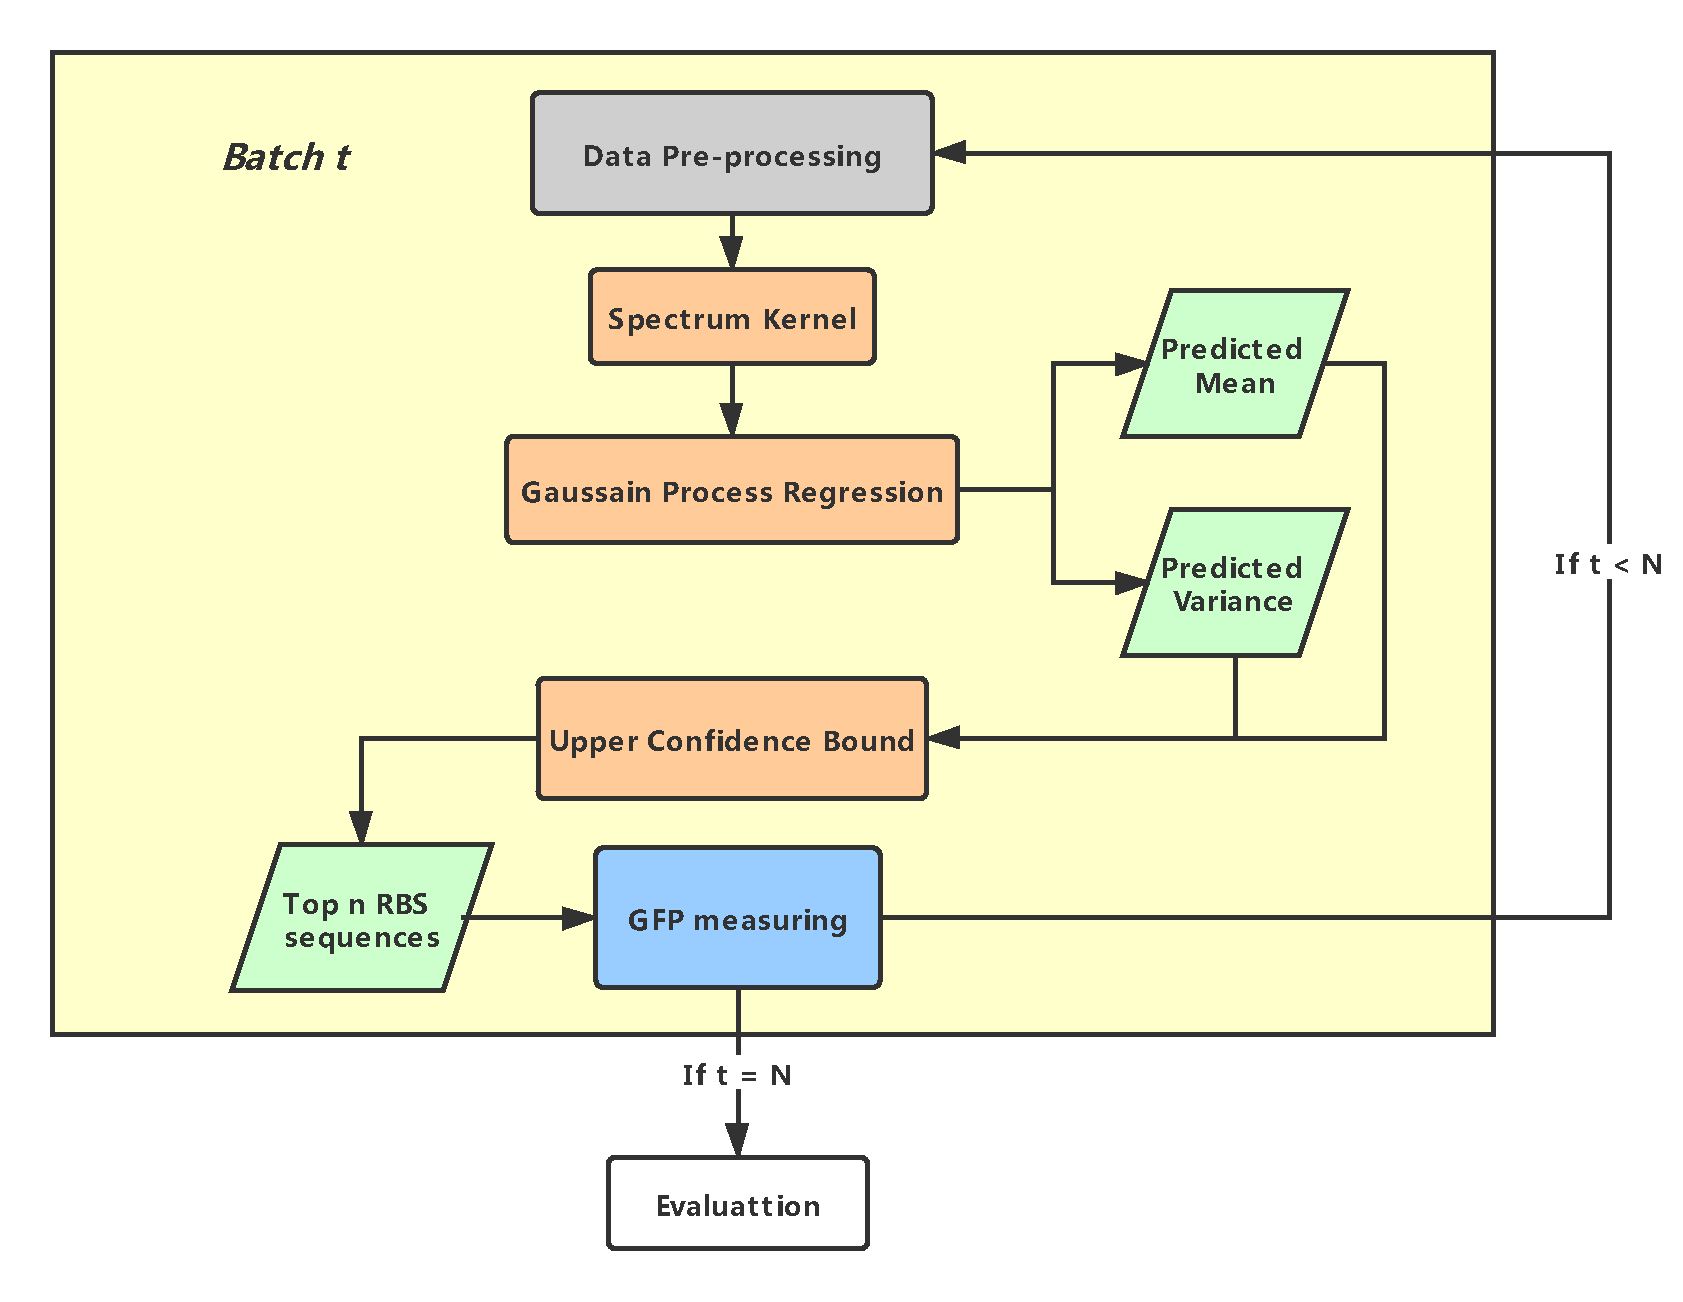
\includegraphics[scale=0.35]{plots/flowchart.pdf}
    \caption{Flowchart of machine learning based experimental design.}
    \label{fig: flowchart of machine learning based experimental design.}
\end{figure}





